\documentclass[conference]{IEEEtran}
\IEEEoverridecommandlockouts
% The preceding line is only needed to identify funding in the first footnote. If that is unneeded, please comment it out.
\usepackage{cite}
\usepackage{amsmath,amssymb,amsfonts}
\usepackage{algorithmic}
\usepackage{graphicx}
\usepackage{textcomp}
\usepackage{xcolor}
\usepackage{algorithm}
\usepackage{array}
\usepackage[utf8]{inputenc}
\usepackage{titlesec}

% Add spacing before sections
\titlespacing{\section}{0pt}{40pt}{20pt}
\titlespacing{\subsection}{25pt}{15pt}{5pt}

\def\BibTeX{{\rm B\kern-.05em{\sc i\kern-.025em b}\kern-.08em
    T\kern-.1667em\lower.7ex\hbox{E}\kern-.125emX}}
\begin{document}

\title{\textit{Optimal Selfish Mining Strategies in Bitcoin: A Comprehensive Summary}\\
}

\author{\IEEEauthorblockN{Panos Lin}
    \IEEEauthorblockA{\textit{Computer Science Department} \\
        \textit{Virginia Commonwealth University}\\
        Richmond, VA \\
        ling8@vcu.edu}
}

\maketitle

\begin{abstract}
    This paper presents a comprehensive summary of "Optimal Selfish Mining Strategies in Bitcoin" by Sapirshtein, Sompolinsky, and Zohar. The original work extends the model of selfish mining attacks in Bitcoin and provides an algorithm to compute optimal strategies for attackers. Our summary covers five key contributions: 
    (1) the generalization and optimization of selfish mining strategies beyond previous approaches, 
    (2) the discovery of a lower profit threshold required for profitable attacks, 
    (3) the evaluation of proposed protocol modifications to mitigate such attacks, 
    (4) the impact of network delays on the viability of selfish mining, and 
    (5) the interaction between selfish mining and double spending attacks. 
    
    Together, these findings demonstrate that Bitcoin's security against selfish mining is more tenuous than previously believed, with significant implications for the cryptocurrency's long-term incentive compatibility.
\end{abstract}

\begin{IEEEkeywords}
    Bitcoin, Selfish Mining, Blockchain Security, Optimization, Double Spending
\end{IEEEkeywords}

\section{Introduction}

\subsection{Background and Motivation}

The security of Bitcoin and other proof-of-work cryptocurrencies relies on miners following the protocol honestly. 
However, in 2014, Eyal and Sirer identified a vulnerability called "selfish mining," 
where miners can increase their relative rewards by deviating from the protocol \cite{eyal2018majority}. 
Their strategy, known as SM1, showed that miners controlling more than a certain threshold of computational power 
could profitably withhold blocks instead of publishing them immediately.

The paper we summarize, "Optimal Selfish Mining Strategies in Bitcoin" by Sapirshtein et al., extends this work by finding optimal selfish mining strategies and examining their implications for Bitcoin's security \cite{sapirshtein2016optimal}. This summary is motivated by the need to understand the full extent of selfish mining vulnerabilities, which could potentially undermine Bitcoin's incentive structure and lead to centralization.

\subsection{Objectives}

This summary paper aims to provide a comprehensive overview of the key findings presented in the original paper, focusing on:

\begin{itemize}
    \item The algorithm for finding $\varepsilon$-optimal selfish mining strategies and its theoretical foundations
    \item The lower profit threshold for selfish mining compared to previous work
    \item The effectiveness of proposed protocol modifications against optimal selfish mining
    \item The impact of network delays on the viability of selfish mining attacks
    \item The relationship between selfish mining and double spending attacks
\end{itemize}


\section{Generalization and Optimization of Selfish Mining}

This section examines how Sapirshtein et al. extended the selfish mining attack model and developed an algorithm to find optimal attack strategies. While the original selfish mining strategy (SM1) demonstrated that Bitcoin is not incentive-compatible, the authors show that even more effective strategies exist and provide a framework for finding them.

\subsection{The Basic Selfish Mining Model}

The selfish mining strategy, first described by Eyal and Sirer \cite{eyal2018majority}, exploits Bitcoin's fork resolution mechanism to increase an attacker's relative revenue. In the standard Bitcoin protocol, miners immediately publish any blocks they discover \cite{nakamoto2008bitcoin}. In selfish mining, attackers strategically withhold blocks to force honest miners to waste computational power on blocks that will eventually be discarded.

Two key parameters characterize the attack model:
\begin{itemize}
    \item $\alpha$: The fraction of the total network hashrate controlled by the attacker (between 0 and 0.5)
    \item $\gamma$: The connectivity parameter representing the fraction of honest miners who would mine on the attacker's blocks in case of a block race (between 0 and 1)
\end{itemize}

In the SM1 strategy, the attacker follows specific rules based on their private chain's lead over the public chain:
\begin{itemize}
    \item When the attacker finds a block, they keep it private instead of publishing it
    \item If the honest miners find a block while the attacker has a one-block lead, the attacker immediately publishes their secret chain, creating a fork
    \item If the honest miners build on the attacker's block during a fork, the attacker gains revenue from the previously withheld block
    \item If the attacker extends their private chain to have a two-block lead, they publish their entire chain, causing honest miners to switch to it and abandoning their work
\end{itemize}

The original analysis showed that SM1 becomes profitable when $\alpha > \frac{1-\gamma}{3-2\gamma}$, which for $\gamma=0$ means attackers need at least 33\% of the network hashrate, and for $\gamma=1$ need just 25\%.

\subsection{Markov Decision Process Formulation}

Sapirshtein et al. generalize the selfish mining problem by formulating it as a Markov Decision Process (MDP). This approach allows them to find optimal strategies rather than analyzing a single predefined strategy.

An MDP consists of states, actions, transition probabilities, and rewards:

\begin{itemize}
    \item \textbf{States}: The state space $(a,h)$ captures the length of the attacker's private chain ($a$) and the length of the honest network's chain ($h$) relative to the last common block.
    
    \item \textbf{Actions}: At each state, the attacker can perform three possible actions:
    \begin{itemize}
        \item \textbf{Adopt}: Abandon their private chain and mine on the public chain
        \item \textbf{Override}: Publish enough blocks to overtake the public chain
        \item \textbf{Match}: Publish exactly enough blocks to match the public chain length
        \item \textbf{Wait}: Continue mining on their private chain without publishing blocks
    \end{itemize}
    
    \item \textbf{Transitions}: Transitions between states occur when either the attacker or honest miners find new blocks. The probability of the attacker finding the next block is $\alpha$, while honest miners find it with probability $1-\alpha$.
    
    \item \textbf{Rewards}: The attacker's reward is measured as the expected fraction of blocks in the main chain that belong to them. The long-term average reward $\rho$ represents the attacker's revenue relative to their resources.
\end{itemize}

\begin{figure}[h!]
    \centering
    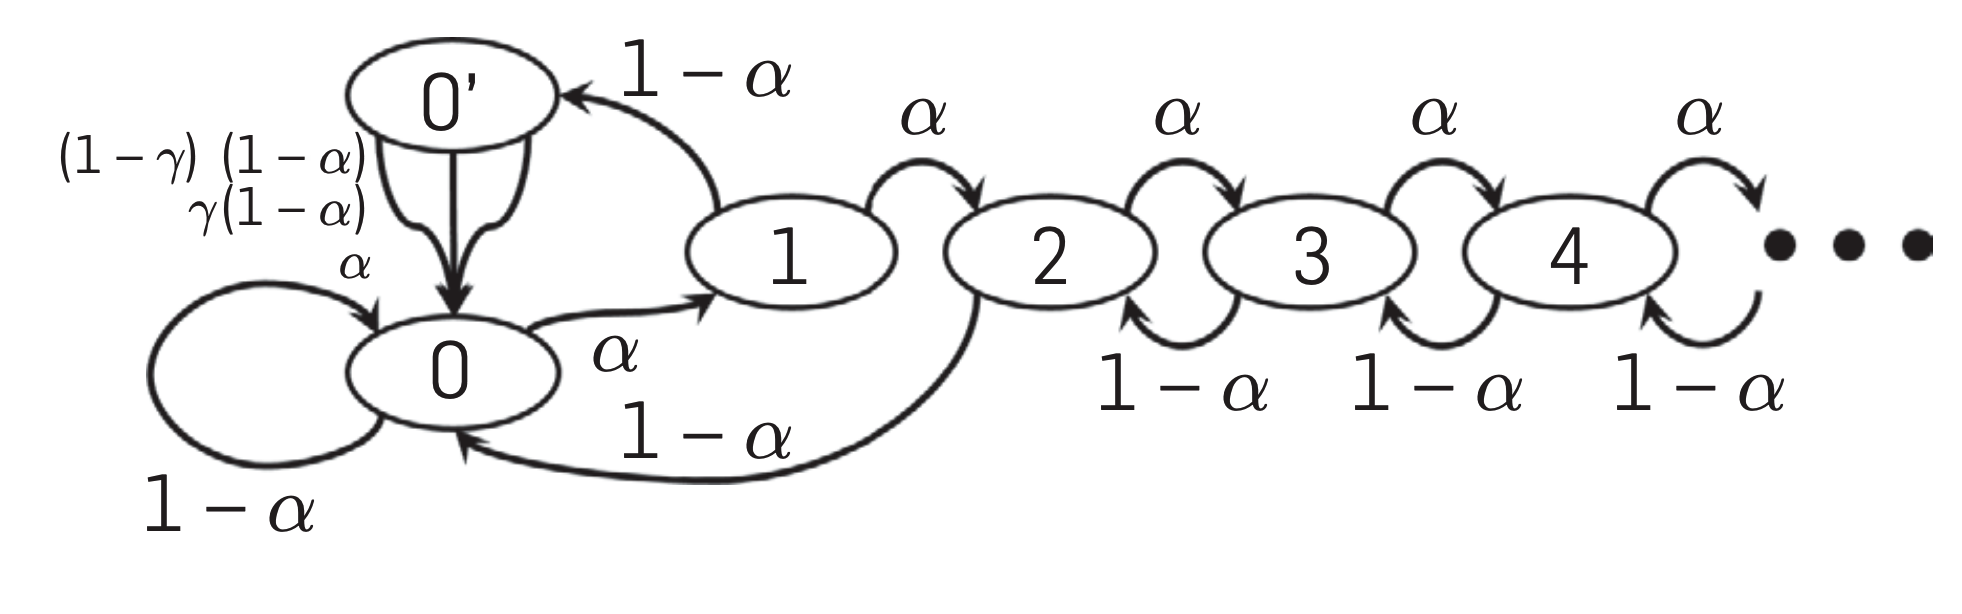
\includegraphics[width=0.5\textwidth]{src/State machine with transition frequencies.png}
    \caption{State machine representation of the SM1}
    \label{fig:state_machine}
\end{figure}

The authors define a policy $\pi$ as a mapping from states to actions. An optimal policy maximizes the attacker's relative revenue. Unlike SM1, which prescribes fixed actions for each state, as shown in Figure \ref{fig:state_machine}, optimal policies can adapt based on precise state configurations.

\subsection{The $\varepsilon$-Optimal Algorithm}

Finding an optimal selfish mining strategy equates to finding an optimal policy for the MDP. The authors develop an algorithm that can compute an $\varepsilon$-optimal policy for any desired precision $\varepsilon > 0$. 

% The algorithm is based on policy iteration with several key improvements:

% \begin{itemize}
%     \item \textbf{State Space Truncation}: Since the state space is theoretically infinite, the authors prove that states can be truncated at a specific threshold while maintaining $\varepsilon$-optimality. They show that states with very large leads $(a \gg h)$ have nearly identical optimal actions.
    
%     \item \textbf{Policy Iteration}: The algorithm alternates between policy evaluation (computing the value of each state under the current policy) and policy improvement (choosing actions that maximize expected value).
    
%     \item \textbf{Convergence Guarantee}: The authors provide mathematical proof that their algorithm converges to an $\varepsilon$-optimal policy in finite time, with bounds on the approximation error.
    
%     \item \textbf{Efficient Implementation}: The algorithm uses dynamic programming techniques to efficiently update state values and policies.
% \end{itemize}

The authors show that their algorithm can find policies with revenues arbitrarily close to the theoretical upper bound of $\frac{\alpha}{1-\alpha}$ when $\gamma = 1$, which represents the maximum theoretical revenue an attacker can achieve.

\subsection{Verification and Implementation}

To validate their approach, the authors implemented both the algorithm and a selfish mining simulator:

\begin{itemize}
    \item \textbf{Simulation Framework}: They created a discrete-event simulation of the Bitcoin network that models block discovery, propagation, and fork resolution.
    
    % \item \textbf{Policy Verification}: All policies generated by the algorithm were tested in the simulator to verify their expected revenue matched theoretical predictions.
    
    \item \textbf{Comparison with SM1}: The simulator allowed direct comparison between the optimal policies and SM1, confirming that optimal policies indeed produce higher revenue in all parameter settings.
    
    \item \textbf{Error Analysis}: The authors analyzed the error bounds of their algorithm and showed that the practical error is typically much smaller than the theoretical bound, especially for reasonable values of $\alpha$ and $\gamma$.
\end{itemize}

The simulation results confirmed that the algorithm successfully finds policies that outperform SM1, particularly for attackers with lower hashrate or better network connectivity. This verification process established the practical viability of the optimization approach and demonstrated that the gap between optimal strategies and SM1 is significant enough to lower the profit threshold for selfish mining attacks.



\section{Lower Profit Threshold for Selfish Mining}

One of the most significant findings of Sapirshtein et al. is that optimal selfish mining strategies can be profitable at lower thresholds of computational power than previously established. This section examines the comparison between optimal strategies and SM1
% , analyzes the revenue curves
% , and discusses the security implications of this lower threshold.

\subsection{Comparison with SM1}

The authors' algorithm generates selfish mining strategies that consistently outperform SM1 across all parameter configurations. As shown in Table \ref{table:comparison_with_sm1}, the key findings from their comparison include:

\begin{table}[h!]
    \centering
    \caption{The revenue of the attacker under SM1 and under the $\varepsilon$-OPT policies, compared to the computed upper bound, for various $\alpha$ and with $\gamma = 0$.}
    \label{table:comparison_with_sm1}
    \begin{tabular}{|c|c|c|c|}
        \hline
        $\alpha$ & $SM1$ & $\varepsilon$-OPT & Upper-Bound \\
        \hline
        $1/3$ & $1/3$ & 0.33705 & 0.33707 \\
        \hline
        0.35 & 0.36650 & 0.37077 & 0.37079 \\
        \hline
        0.375 & 0.42118 & 0.42600 & 0.42604 \\
        \hline
        0.4 & 0.48372 & 0.48866 & 0.48904 \\
        \hline
        0.425 & 0.55801 & 0.56808 & 0.57226 \\
        \hline
        0.45 & 0.65177 & 0.66891 & 0.70109 \\
        \hline
        0.475 & 0.78254 & 0.80172 & 0.90476 \\
        \hline
    \end{tabular}
\end{table}

\begin{itemize}
    \item For all values of $\alpha$ and $\gamma$, the optimal strategy either matches or exceeds the revenue of SM1.
    
    \item The improvement over SM1 is most pronounced for miners with computational power near the original profitability threshold.
    
    \item The gap between SM1 and optimal strategies narrows as $\alpha$ increases, indicating that SM1 approaches optimality for attackers with significant computational resources.
    
    \item For smaller attackers (those with $\alpha$ close to the profit threshold), optimal strategies involve more nuanced decisions on when to adopt the honest chain versus when to continue selfish mining.
\end{itemize}

The performance difference arises primarily from the optimal strategy's more sophisticated approach to managing the private chain under specific state configurations. Where SM1 follows fixed rules, optimal strategies dynamically adjust based on the precise state of both chains.

% \subsection{Revenue Analysis}

% The authors present comprehensive revenue analysis through a series of graphs comparing honest mining, SM1, and the $\varepsilon$-optimal policies. Key insights from this analysis include:

% \begin{itemize}
%     \item The revenue of an attacker ($\rho$) under optimal selfish mining is bounded by $\frac{\alpha}{1-\alpha}$, which represents the maximum theoretical revenue achievable when $\gamma = 1$.
    
%     \item When $\gamma = 0$ (worst network connectivity), the profit threshold drops from approximately 33\% (for SM1) to around 32\% with optimal strategies.
    
%     \item For $\gamma = 0.5$ (moderate connectivity), the threshold decreases from approximately 30\% to about 27\%.
    
%     \item When $\gamma = 1$ (ideal connectivity), the threshold drops from 25\% to approximately 23.2\%.
% \end{itemize}

% Figure 1 in the original paper clearly demonstrates these differences, showing the revenue curves of honest mining, SM1, and optimal strategies for various $\gamma$ values. The curves illustrate that optimal strategies consistently yield higher revenue than SM1, particularly in the threshold regions where selfish mining first becomes profitable.

% The authors define the profit threshold as the value of $\alpha$ at which the relative revenue from selfish mining equals that from honest mining ($\rho = \alpha$). Their analysis indicates that optimal strategies lower this threshold across all connectivity scenarios, making selfish mining viable for attackers with fewer resources than previously thought necessary.

% \subsection{Implications for Bitcoin Security}

% The discovery of a lower profit threshold for selfish mining has several significant implications for Bitcoin's security model:

% \begin{itemize}
%     \item \textbf{Reduced Security Margin}: The lower threshold indicates that Bitcoin's security margin against selfish mining is narrower than previously believed. This is particularly concerning as mining pools often control significant portions of the network hashrate.
    
%     \item \textbf{Incentive Incompatibility}: The results strengthen the argument that Bitcoin's protocol is not incentive-compatible, as miners with even less computational power than previously thought can benefit from deviating from the protocol.
    
%     \item \textbf{Mining Centralization Pressure}: The existence of more efficient selfish mining strategies could accelerate mining centralization. Miners who successfully execute selfish mining become more profitable, potentially attracting more computational power and further increasing their advantage.
    
%     \item \textbf{Practical Attack Viability}: While the improvement over SM1 is modest (roughly 1-2 percentage points in the threshold), this difference could be significant in practice. As mining pools routinely approach or exceed 20\% of the network hashrate, the difference between a 25\% and 23.2\% threshold could determine whether an attack is viable.
% \end{itemize}

% These findings suggest that the security of Bitcoin against selfish mining is more tenuous than previously understood. Although the reduction in threshold is not dramatic, it narrows the safety margin and might bring the attack within reach of large mining entities, especially those with favorable network connectivity.

% The authors note that these results can be viewed from both negative and positive perspectives: negatively, as they demonstrate greater vulnerability; positively, as they establish tighter lower bounds on the computational power required for profitable attacks, helping to quantify the actual security margin of the system.

\section{Evaluation of Protocol Modifications}

This section examines the authors' analysis of protocol modifications proposed to mitigate selfish mining, particularly the uniform tie-breaking rule suggested by Eyal and Sirer.

\subsection{The Uniform Tie-Breaking Rule}

Eyal and Sirer proposed a simple countermeasure against selfish mining: when miners encounter competing chains of equal length, they should choose which chain to extend uniformly at random, rather than defaulting to the first-seen chain. This modification aims to reduce the attacker's advantage during "block races" by decreasing the value of the $\gamma$ parameter.

Under the current Bitcoin protocol, when a selfish miner publishes a previously withheld block that creates a fork of equal length with the honest chain, miners typically extend the chain they received first (usually the honest chain). With uniform random selection between equal-length chains, the attacker has a 50\% chance of having their chain extended regardless of propagation advantages.

\subsection{Effectiveness Against Optimal Strategies}

Sapirshtein et al. evaluated this countermeasure by computing optimal selfish mining strategies against the modified protocol. Their findings:

\begin{itemize}
    \item The modification is somewhat effective against strong attackers (high $\alpha$), reducing their maximum potential revenue
    \item For $\gamma = 1$, the profit threshold increases from approximately 23.2\% to 25\% 
    \item The uniform selection rule effectively forces $\gamma = 0.5$ for block races, reducing the impact of network advantages
\end{itemize}

However, contrary to Eyal and Sirer's conjecture that this modification would increase the profit threshold to 25\% for all $\gamma$ values, the authors found that attackers with less than 25\% of computational power can still profit from selfish mining under certain conditions.

\subsection{Unexpected Benefits for Medium-Sized Attackers}

The authors discovered a surprising result: the uniform tie-breaking rule actually benefits medium-sized attackers with poor network connectivity. Specifically:

\begin{itemize}
    \item For attackers with low $\gamma$ values (poor network connectivity), the uniform selection rule provides an artificial improvement in effective connectivity
    \item This effect is particularly pronounced for attackers with $\alpha$ between 25\% and 32\%
    \item Such attackers gain higher revenue under the modified protocol than under the original one
\end{itemize}

This counterintuitive result demonstrates that protocol modifications may have unexpected consequences when attackers employ optimal strategies rather than fixed approaches like SM1.

\subsection{Implications for Protocol Design}

The analysis of the uniform tie-breaking rule offers important insights for protocol design:

\begin{itemize}
    \item Protocol modifications require rigorous analysis against optimized adversarial strategies, not just specific attack vectors
    \item Simple fixes may have unintended consequences that benefit certain classes of attackers
    \item The uniform tie-breaking rule is not a comprehensive solution to selfish mining
    \item More fundamental protocol changes may be necessary to address selfish mining vulnerabilities
\end{itemize}

The authors suggest that effective countermeasures should consider both the computational power and network connectivity of potential attackers, as improvements in one dimension may offset vulnerabilities in the other.

\section{Impact of Network Delays}

This section will cover how network propagation delays affect the viability of selfish mining attacks.

\subsection{Network Delay Model}

[Describe how the authors model network delays in their analysis.]

\subsection{Vanishing Profit Threshold}

[Explain the paper's finding that, with network delays, the profit threshold for selfish mining vanishes.]

\subsection{Small Miner Advantage}

[Discuss how even miners with very small hashrates can profit from selfish mining under realistic network conditions.]

\subsection{Real-World Implications}

[Address what these findings mean for Bitcoin in practice, given that the real network does experience propagation delays.]

\section{Interaction with Double Spending}

This section will explore the connection between selfish mining and double spending attacks.

\subsection{Double Spending Attack Mechanics}

[Provide a brief explanation of double spending attacks in Bitcoin.]

\subsection{Cost-Free Double Spending}

[Explain the paper's finding that selfish miners can perform double spending attacks at no additional cost.]

\subsection{Challenges to Nakamoto's Security Analysis}

[Discuss how these findings undermine aspects of Satoshi Nakamoto's original security analysis for Bitcoin.]

\subsection{Comprehensive Threat Model}

[Present the more comprehensive threat model that emerges when considering both selfish mining and double spending together.]

\section{Conclusion}

The original paper makes significant contributions to understanding Bitcoin's security against selfish mining attacks. By finding optimal selfish mining strategies, the authors demonstrated that the profit threshold is lower than previously thought, protocol modifications may have unexpected effects, network delays eliminate the threshold entirely, and selfish mining enables cost-free double spending.

These findings highlight the need for continued research into Bitcoin's incentive compatibility and security model. Future work could focus on developing more robust protocol modifications, exploring the practical feasibility of these attacks in the wild, and addressing the fundamental tension between network efficiency and security in decentralized consensus systems.

\bibliographystyle{unsrt}
\bibliography{ref}

\end{document}